\section{Experimental design}
\label{sec:design}
\paragraph{Data and sampling model.} Real data are the nine example sets of \texttt{ppi-python} 0.2.3~\citep{ppipython} (labels $Y$ and predictions $f$): galaxies (spiral indicator; \citealt{willett2013galaxyzoo2}), forest, AlphaFold, gene expression, census income (income, continuous; \citealt{ding2021retiring}), ballots, census healthcare and education (appendix), and plankton (distribution-shift stress test). Each dataset's pool is the population and $\theta$ is the pool mean of $Y$. Labeled and unlabeled records are drawn independently and i.i.d.\ \emph{with replacement} from the pool, so the fraction of the pool used does not enter, with $n\in\{50,100,200,400,1000\}$ capped at pool$/5$ (forest and ballots: $n\le200$) and $N=20n$; a second sweep varies $N\in\{n,5n,20n,20000\}$. For ballots, whose real unlabeled split has no labels, the pool is its 1027 labeled records. For plankton the labeled records come from the 2013 pool and the unlabeled predictions from 2014, with $\theta$ the mean of the 2014 labels; the control draws both from 2013. A forest ablation draws labeled records without replacement. Synthetic populations with known truth (Appendix~\ref{app:synth}) vary the nonlinearity $\kappa$ of $E[Y\mid f]$ ($\tanh$, quadratic, and a binary outcome with an overconfident classifier), $n$, $N/n$, the signal-to-noise ratio and the noise tail.

\paragraph{Replication and uncertainty.} Every cell uses $R=2000$ replicates, and all methods see the same draws within a replicate, so width comparisons are paired. Coverage is reported with its Wilson interval~\citep{wilson1927}; the Monte-Carlo standard error is $\le0.0049$ near $0.95$. Width is the paired geometric-mean ratio to M3 with a 95\% percentile bootstrap interval over replicates. A cell is flagged below nominal (bold in tables) when the Wilson upper bound is $<0.95$. We make a coverage claim only for a pattern across neighbouring $n$ or datasets, not for single cells; no cell-level $p$-values are computed, and the 26 primary real cells and the synthetic cells are not corrected for multiplicity. Seeds are derived from (dataset, $n$, $N$) in a final space disjoint from the development space used to choose M4 and M5. Tables~\ref{tab:methods} and the reproduction notes list methods, seeds, commands and run times.

\begin{table}[t]
\caption{Methods compared. All use only the labeled $(Y,f)$ and the unlabeled $f$.}
\label{tab:methods}
\centering\scriptsize
\adjustbox{max width=\linewidth}{\begin{tabular}{llp{3.4cm}p{2.6cm}l}
\toprule
 & Method & Point estimate & Information used & Critical value \\
\midrule
M1 & classical & mean of $Y$ on the $n$ labeled & labels only & $z$ \\
M2 & PPI & $\bar f_{\rm unl}+\overline{(Y-f)}_{\rm lab}$ & $(Y,f)$ labeled, $f$ unlabeled & $z$ \\
M3 & PPI++ (\texttt{ppi\_py} 0.2.3, reference) & power-tuned $\hat\lambda\in[0,1]$ & same as M2 & $z$ \\
M4 & isotonic-calibrated PPI++ & PPI++ on a score $\hat g(f)$ learned on the labels, 5-fold cross-fitted & same as M2 (covariates not used) & $z$ \\
M5 & small-$n$ corrections & M3 with delete-one jackknife s.e.; M4 with $t_{n-1}$ & same as M2 & $t_{n-1}$ \\
\bottomrule
\end{tabular}
}
\end{table}

\section{Results}
\label{sec:results}
\subsection{On the real datasets the fixed-input ceiling is almost reached by PPI++}
\label{sec:real}
Table~\ref{tab:datasets} gives, for each dataset, the population quantities that enter the ceiling~\eqref{eq:floor}. $E[Y\mid f]$ is nearly affine in $f$ on all of them: $|R^2_{\rm cal}-\rho^2|<0.01$ everywhere (the cross-fitted estimate can fall slightly below $\rho^2$, as on forest), so the predicted asymptotic width ratio (a floor estimated with cross-fitted isotonic maps, hence occasionally slightly above $1$, as on forest and ballots) of a calibrated interval to M3 is within $\pm0.5\%$ of $1$ for seven of the nine sets, $0.983$ for census income and $0.964$ for gene expression. Most of these two gains is the clip, not calibration: against \emph{unclipped} PPI++ the ratios are $0.998$ and $0.993$, because there the optimal $\hat\lambda$ exceeds one and M3 clips it.

Figure~\ref{fig:real} shows the measured effect of calibration. M4 is wider than M3 in 24 of the 26 primary cells (paired ratio $1.02$--$1.11$ at $n=50$, $1.006$--$1.046$ at $n=200$, $0.995$--$1.025$ at $n=400$ and $0.979$--$1.009$ at $n=1000$). The two exceptions are gene expression at $n=400$ and $1000$ (ratios $0.995$ and $0.979$); unclipped PPI++ with an affine score (\texttt{ppipp\_nc}) gives $0.979$ and $0.974$ in the same cells, so the gain there is the removal of the clip, not calibration. M2 (PPI, $\lambda=1$) is within $\pm2.5\%$ of M3 everywhere, and M1 is $1.2$ to $3.7$ times wider (Appendix Table~\ref{tab:realwidth}). Table~\ref{tab:regimes} summarises the regimes. Hence \emph{no calibrated-score interval of the kind studied is appreciably shorter than PPI++ on these datasets}, consistent with the ceiling; the two exceptions below are the removal of the clip.

The excess width of M4 over the ceiling is the plug-in cost of learning $\hat g$ (Figure~\ref{fig:plugin}): measured/predicted $-1$ is $1.4$--$12.6\%$ at $n=50$, $1.7$--$4.3\%$ at $n=400$ and $0.8$--$2.4\%$ at $n=1000$ (smallest on ballots), and on galaxies and forest it grows with $N/n$, as expected if a larger unlabeled set raises the optimal weight on $\hat g$ (we did not test this; on gene expression and census income it does not grow) (galaxies, $n=100$: $1.020$, $1.052$ and $1.059$ for $N=n$, $20n$ and $200n$).



\begin{table}[t]
\caption{Population quantities behind the ceiling~\eqref{eq:floor} for each dataset (pool values); the last two columns are the asymptotic width ratio of an isotonic-calibrated interval to M3 without estimation cost, at $N=20n$.}
\label{tab:datasets}
\centering\scriptsize
\adjustbox{max width=\linewidth}{\begin{tabular}{lrrrrrr}
\toprule
Dataset & Pool size & $\mathrm{Var}(Y)$ & $\rho^2$ & $R^2_{\rm cal}$ & floor ratio, $n=100$ & floor ratio, $n=400$ \\
\midrule
Galaxies & 16\,743 & 0.1921 & 0.549 & 0.547 & 1.001 & 1.001 \\
Forest & 1\,596 & 0.1286 & 0.289 & 0.281 & 1.005 & 1.005 \\
AlphaFold & 10\,802 & 0.1459 & 0.664 & 0.665 & 0.999 & 0.999 \\
Gene expression & 61\,150 & 19.28 & 0.928 & 0.930 & 0.964 & 0.964 \\
Census income & 380\,091 & $5.758\times10^{9}$ & 0.369 & 0.372 & 0.983 & 0.983 \\
Census healthcare & 318\,215 & 0.2208 & 0.500 & 0.500 & 1.000 & 1.000 \\
Census education & 318\,215 & 19.23 & 0.392 & 0.392 & 1.000 & 1.000 \\
Ballots & 1\,027 & 0.2336 & 0.963 & 0.963 & 1.004 & -- \\
Plankton & 421\,238 & 0.1159 & 0.699 & 0.699 & 1.000 & 1.000 \\
\bottomrule
\end{tabular}
}
\end{table}

\begin{figure}[t]
\centering
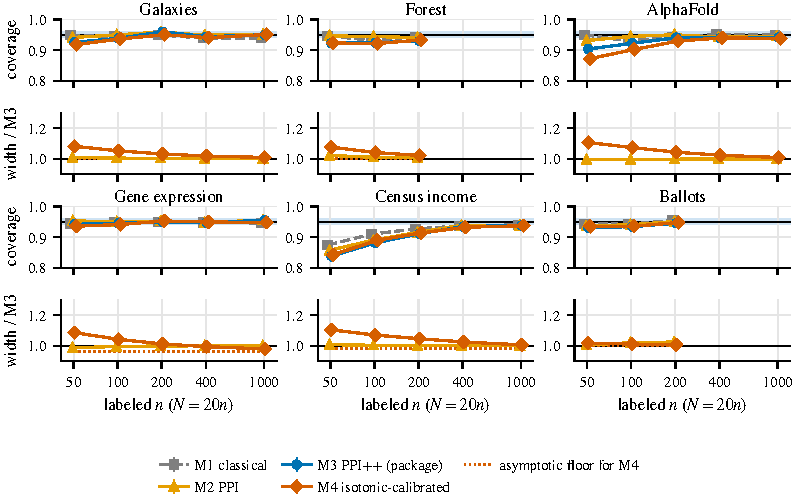
\includegraphics[width=\linewidth]{../figures/real_main.pdf}
\caption{Coverage (top rows, Wilson 95\% intervals; shaded band: range of a nominally covering method's Monte-Carlo estimate) and paired width ratio to M3 (bottom rows; 95\% bootstrap interval; dotted: asymptotic ratio for M4 from population quantities) on six real datasets, $N=20n$, $R=2000$.}
\label{fig:real}
\end{figure}

\begin{figure}[t]
\centering
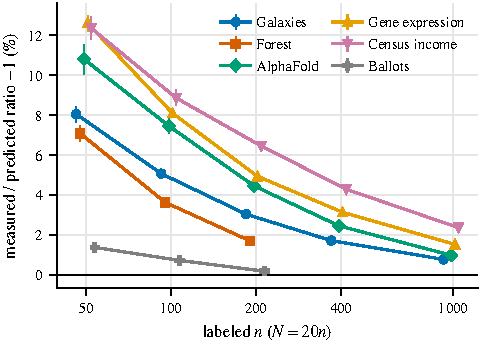
\includegraphics[width=\linewidth]{../figures/plugin_cost.pdf}
\caption{Plug-in cost of M4: measured over predicted width ratio minus one, versus $n$ ($N=20n$).}
\label{fig:plugin}
\end{figure}

\begin{table}[t]
\caption{Regimes by dataset (real rows: 36 cells in all; synthetic rows: the 23 $\kappa$- and $n$-sweep cells at SNR $1$): number of cells where M4 is narrower, indistinguishable or wider than M3 (paired 95\% interval), the range of the ratio, and the number of cells below nominal for M3 and M4.}
\label{tab:regimes}
\centering\scriptsize
\adjustbox{max width=\linewidth}{\begin{tabular}{lrrrrrrrr}
\toprule
Cells & \# & M4 narrower & indistinguishable & M4 wider & smallest ratio & largest ratio & M3 undercovers & M4 undercovers \\
\midrule
Galaxies & 5 & 0 & 0 & 5 & 1.009 & 1.082 & 2 & 2 \\
Forest & 3 & 0 & 0 & 3 & 1.022 & 1.076 & 3 & 3 \\
AlphaFold & 5 & 0 & 0 & 5 & 1.009 & 1.107 & 3 & 5 \\
Gene expression & 5 & 2 & 0 & 3 & 0.979 & 1.086 & 0 & 1 \\
Census income & 5 & 0 & 0 & 5 & 1.006 & 1.104 & 5 & 5 \\
Census healthcare & 5 & 0 & 0 & 5 & 1.009 & 1.073 & 1 & 2 \\
Census education & 5 & 0 & 0 & 5 & 1.013 & 1.092 & 3 & 2 \\
Ballots & 3 & 0 & 0 & 3 & 1.006 & 1.018 & 2 & 2 \\
synthetic, $\kappa=0$ & 3 & 0 & 0 & 3 & 1.017 & 1.060 & 1 & 0 \\
synthetic, tanh/quad, $\kappa>0$ & 16 & 15 & 1 & 0 & 0.864 & 0.998 & 4 & 3 \\
synthetic, binary, $\kappa>0$ & 4 & 0 & 0 & 4 & 1.015 & 1.018 & 3 & 3 \\
\bottomrule
\end{tabular}
}
\end{table}

\subsection{When shortening is possible: nonlinear $E[Y\mid f]$}
\label{sec:synth}
On synthetic populations where $E[Y\mid f]=\sqrt{1-\kappa}\,f+\sqrt\kappa\,h(f)$ the ceiling is lower and M4 reaches part of it (Figure~\ref{fig:syn}). With $\kappa=0$ (affine) M4 is $6\%$ wider than M3 at $n=100$, $N=20n$, the pure cost of cross-fitting; an affine cross-fitted map is similar ($1.03$). For a saturating $h=\tanh$ the ratio is $0.951$ at $\kappa=0.75$ against a ceiling of $0.897$. For a quadratic $h$ (a U-shape that no affine score can use) the ratio is $0.912$ at $\kappa=0.75$ (ceiling $0.773$) and $0.930$ at $\kappa=0.5$ (ceiling $0.830$), and falls to $0.86$ at $n=1000$ and $0.79$ at SNR $=4$; the measured ratio is above the ceiling in every one of the 45 synthetic cells (mean log gap $0.07$, range $0.01$--$0.27$; log-correlation $0.88$ between predicted and measured ratios). For the binary outcome with a miscalibrated classifier M4 is never narrower than M3 except at $n=400$, $\kappa=0$ (ratio $0.989$), because $E[Y\mid f]$ is smooth and close to affine in the score's range. Isotonic regression cannot represent a U-shape: on the quadratic population the final-run spline calibrator (not selected as M4) reaches $0.83$ at $\kappa=1$ against the ceiling $0.73$, while isotonic gives $0.95$ (Appendix~\ref{app:synth}; the choice of M4 was fixed before these runs, so this is a post-hoc ablation). With $\kappa>0$ the gain is therefore bounded by the nonlinearity, larger with more labels (plug-in cost shrinks), more unlabeled data and cleaner labels.

\begin{figure}[t]
\centering
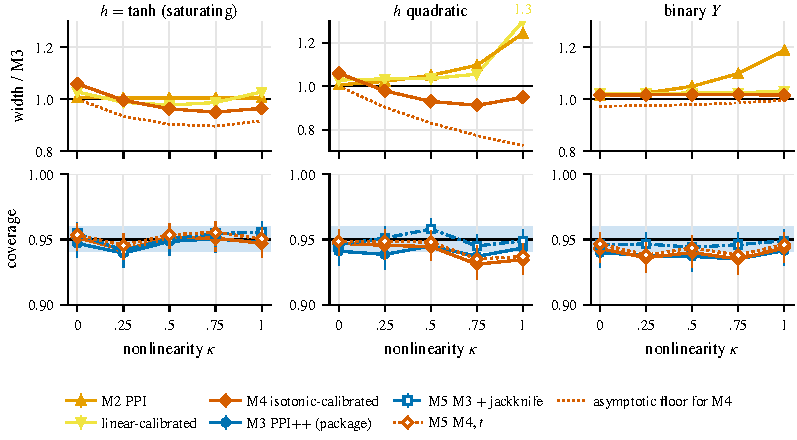
\includegraphics[width=\linewidth]{../figures/synthetic_kappa.pdf}
\caption{Synthetic populations: paired width ratio to M3 and coverage versus the nonlinearity $\kappa$ ($n=100$, $N=20n$, SNR $=1$, $R=2000$). Dotted: asymptotic ceiling for M4.}
\label{fig:syn}
\end{figure}

\subsection{Validity at small $n$: the plug-in interval undercovers, and the cure costs width}
\label{sec:validity}
M3 undercovers at small $n$ in a consistent pattern (Table~\ref{tab:regimes}, Appendix Table~\ref{tab:cov} for $n=100,400$ and \texttt{tab\_real\_full.csv} for all cells; Figures~\ref{fig:real} and~\ref{fig:corr}): at $n=50$ the coverage is $0.904$ (AlphaFold), $0.838$ (census income), $0.923$ (forest) and $0.925$ (galaxies), and in 15 of the 26 primary cells the Wilson upper bound is below $0.95$. M4 has lower coverage on AlphaFold ($n=100$: $0.902$ against $0.922$) and galaxies and comparable coverage elsewhere (all cells: \texttt{tab\_real\_full.csv} in the delivered tables). The delete-one jackknife with $t_{n-1}$ (M5 on M3) raises these to $0.954$, $0.868$, $0.942$ and $0.949$ at $n=50$ for $10$--$15\%$ more width ($2$--$4\%$ at $n=200$); $t_{n-1}$ alone on M4 helps less (AlphaFold $n=50$: $0.880$). Census income stays below $0.95$ up to $n=400$ for every method, including the classical $z$ interval ($0.874$ at $n=50$); we suspect skewed income labels but did not test this. A bootstrap ablation (Appendix Table~\ref{tab:boot}) shows that a percentile bootstrap of PPI++ does not repair coverage, while a studentized bootstrap does so in most cells except census income, at $2$--$24\%$ greater width ($14$--$49\%$ on census income, which it does not repair). The conformal baseline of \texttt{ppi-python} is the whole real line unless $n\ge N/\alpha-1$, which never holds at $N=20n$, so it gives no finite interval in our design.

\begin{figure}[!t]
\centering
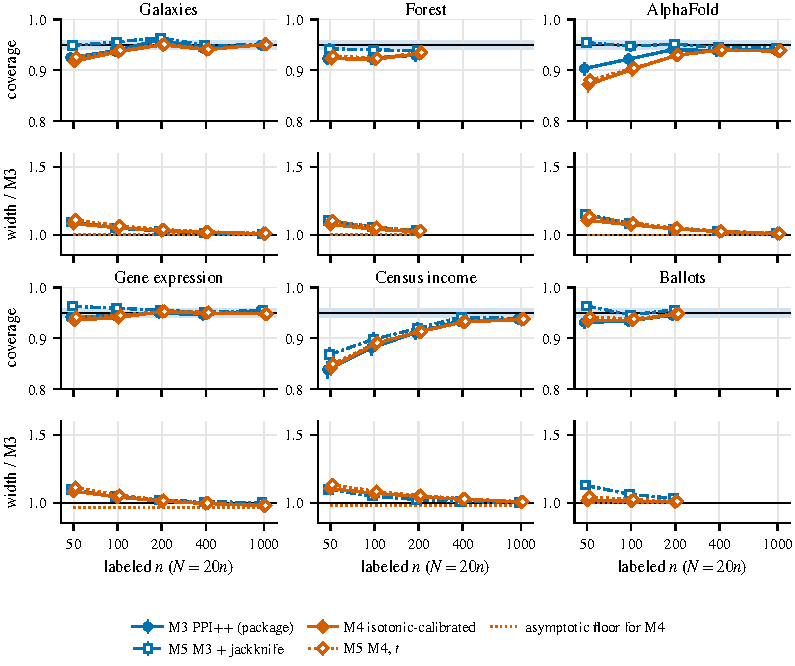
\includegraphics[width=\linewidth]{../figures/real_correction.pdf}
\caption{Small-$n$ corrections on the six primary real datasets: M3, M5 on M3 (jackknife, $t$), M4 and M5 on M4 ($t$). Layout as in Figure~\ref{fig:real}.}
\label{fig:corr}
\end{figure}

\subsection{Distribution shift breaks the optimal-weight intervals}
\label{sec:shift}
On plankton, labeled records from 2013 and unlabeled predictions from 2014 differ in distribution (mean $Y$ $0.134$ versus $0.071$). The classical interval's coverage falls to $0.00$ at $n=1000$ (bias), while M2, M3 and the jackknife M5 keep $0.94$--$0.97$ (Figure~\ref{fig:shift}). Every variant with an unclipped or calibrated $\hat\lambda$, M4 included, degrades with $n$ (M4 coverage $0.90$, $0.80$, $0.67$, $0.49$, $0.18$ at $n=50,100,200,400,1000$; at $n=400$ unclipped PPI++ $0.49$, within-2013 control $0.93$--$0.94$). A direct check (\texttt{code/src/shift\_lambda\_check.py}) shows why: under shift the variance of the unlabeled (2014) scores is smaller than that of the 2013 scores ($0.062$ versus $0.114$), so $\hat\lambda\approx1.40$ in $82$--$100\%$ of draws (control: $0.80$; $R=300$ draws per $n$), which puts negative weight on the labeled-minus-unlabeled prediction contrast that carries the shift; M3 survives only because the package clips $\hat\lambda$ at $1$. An affine cross-fitted score fails equally, so calibration itself is not the cause.

\begin{figure}[!t]
\centering
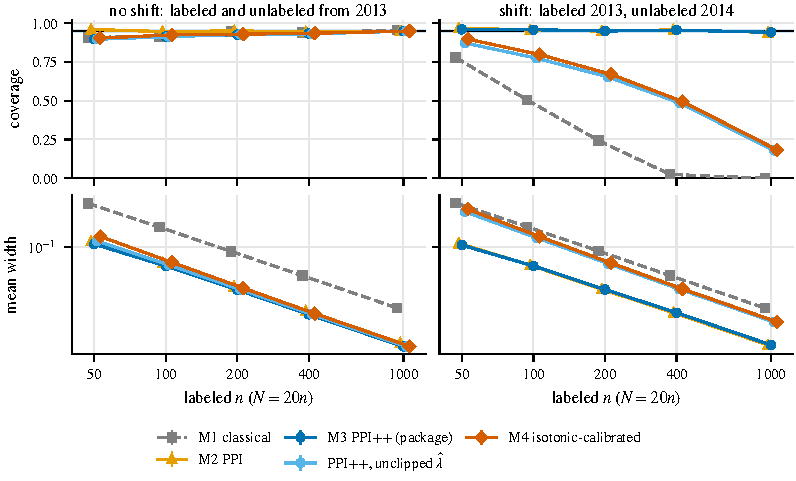
\includegraphics[width=\linewidth]{../figures/plankton_shift.pdf}
\caption{Plankton: labeled 2013 versus unlabeled 2014 (shift) against a within-2013 control; coverage versus $n$ ($R=2000$).}
\label{fig:shift}
\end{figure}
